\documentclass[11pt]{beamer}

% Theme
\usetheme{Madrid}
\usecolortheme{beaver}
\usefonttheme{professionalfonts}

% Packages
\usepackage[T1]{fontenc}
\usepackage[utf8]{inputenc}
\usepackage{lmodern}
\usepackage{amsmath,amssymb,amsthm}
\usepackage{graphicx}
\usepackage{hyperref}
\usepackage{tikz}
\usetikzlibrary{arrows,positioning}
\usepackage{listings}
\usepackage{caption}
\usepackage{subcaption}
\usepackage{epstopdf}
\usepackage{mathrsfs}
\usepackage{booktabs}
\usepackage{pgfplots}
\pgfplotsset{compat=1.17}

% Bibliography
% \usepackage{biblatex}
% \addbibresource{refs.bib}

% Code style
\lstset{
  basicstyle=\ttfamily\small,
  keywordstyle=\color{blue},
  commentstyle=\color{gray},
  stringstyle=\color{red!60!black},
  showstringspaces=false,
  breaklines=true,
  frame=single
}

% Shorthands
\newcommand{\E}{\mathbb{E}}
\newcommand{\mus}{\mu^{\star}}
\newcommand{\muh}{\widehat{\mu}}
\newcommand{\LCB}{\mathrm{LCB}}
\newcommand{\UCB}{\mathrm{UCB}}
\newcommand{\Vinv}{V^{-1}}
\newcommand{\logT}{\log T}

% Title
\title[CS6007 Project]{Contextualizing Fairness: Extending $p$-Mean Social Welfare to Linear Bandits}

% Show ONLY names in the bottom-left footer via the optional [] argument
\author[Kunj, Dhruvraj]{%
  \textbf{Presented by:}\\
  \begin{tabular}{rl}
    \textcolor{blue}{Kunj Bhesaniya (23B0995)} & Dept. of CSE \\
    \textcolor{blue}{Dhruvraj Merchant (23B1041)} & Dept. of CSE \\
  \end{tabular}\\[1em]
  \textbf{Course:} CS6007:Multi-Agent Machine Learning\\[0.3em]
  \textbf{Instructor:} Prof.\ Avishek Ghosh
}

\institute[IIT Bombay]{IIT Bombay}
% \date{\small August 2025}

% Small logo on each frametitle (top-right)
\addtobeamertemplate{frametitle}{}{%
  \begin{tikzpicture}[remember picture,overlay]
    \node[anchor=north east, xshift=0.2cm, yshift=0.4cm] at (current page.north east) {%
      
\includegraphics[height=1.2cm]{CS6007_Slide_Format/iitb_logo.png}%
    };
  \end{tikzpicture}%
}

\begin{document}

% Title slide with faint logo background
\usebackgroundtemplate{%
  \tikz[remember picture,overlay] \node[opacity=0.2] at ([yshift=-2cm]current page.center) {%
    
\includegraphics[width=0.6\paperwidth]{CS6007_Slide_Format/iitb_logo.png}%
  };
}
\begin{frame}
  \titlepage
\end{frame}
\usebackgroundtemplate{} % clear background

% Outline
\begin{frame}{Outline}
  \setbeamertemplate{section in toc}[sections numbered]
  \tableofcontents
\end{frame}

%==================================================
\section{Problem Statement and Motivation}
%==================================================

\begin{frame}{Motivation: From Utilitarian Bandits to $p$-Mean Welfare}
  \small
  \begin{itemize}
    \item \textbf{Sequential Multi-User Bandits:} Round $t \in [T]$ serves a distinct user (e.g., patient in clinical trial). Learner pulls arm $I_t \in [k]$ with unknown mean $\mu_i \ge 0$ ($\sigma^2$-sub-Gaussian); $\mus = \max_i \mu_i$.
    \item \textbf{Failure of Utilitarian Regret:} Standard average regret,
          $AR_T = \mus - \frac{1}{T}\sum_{t=1}^{T}\E[\mu_{I_t}]$,
          maximizes \emph{total} return but is blind to inequality: it can starve unlucky users for aggregate gain.
    \item \textbf{Fair Social Welfare via Power Means:} To protect users, replace arithmetic mean with the \emph{power mean} ($\mu_i \ge 0$ ensures well-defined welfare utilities):
          \[
            R_T^{p} \;=\; \mus - \Big(\tfrac1T\sum_{t=1}^{T}(\E[\mu_{I_t}])^p\Big)^{1/p},
            \qquad
            NR_T \;=\; \mus - \Big(\prod_{t=1}^{T}\E[\mu_{I_t}]\Big)^{1/T}
          \]
  \end{itemize}

  \begin{columns}[T]
    \begin{column}{0.50\textwidth}
      \footnotesize
      \textbf{Fairness Spectrum ($p \le 1$ \cite{moulin2004,sarkar2025}):}
      \begin{itemize}
        \item $p = 1$: Utilitarian ($R^1_T = AR_T$)
        \item $p = 0$: Nash Social Welfare
        \item $p \to -\infty$: Rawlsian (worst-off user)
      \end{itemize}
    \end{column}
    \begin{column}{0.48\textwidth}
      \footnotesize
      \textbf{Key Properties \& Hardness:}
      \begin{itemize}
        \item $R_T^{p}\ \uparrow\ \text{as } p\downarrow$, with $NR_T \ge AR_T$
        \item Smaller $p$ penalizes low rewards more: \textbf{strictly higher fairness, harder learning}.
      \end{itemize}
    \end{column}
  \end{columns}
\end{frame}

\begin{frame}{Comparison with Prior Work}
  \small
  \begin{itemize}
    \item \textbf{The Core Challenge:} A single near-zero pull collapses $p$-mean welfare ($p \le 0$). Standard UCB fails; prior algorithms relied on heavy assumptions to prevent collapse.
  \end{itemize}

  \vspace{2pt}
  \centering
  \small
  \setlength{\tabcolsep}{4pt}
  \begin{tabular}{lccc}
    \toprule
    Algorithm & $p\in[0,1]$ & $p\in[-1,0)$ & $p<-1$ \\
    \midrule
    Barman et al.\ (2023) & $O(\sqrt{k/T})$ \scriptsize{($p=0$)} & -- & -- \\
    Krishna et al.\ (2025) & $O(\sqrt{k/T})$ & $O(k^{3/4}T^{-1/4})$ & $O(k^{1/2}T^{-1/(4|p|)})$ \\
    \textbf{Welfarist-UCB} & $\mathbf{\tilde{O}(\sqrt{k/T})}$ & $\mathbf{\tilde{O}(k/\sqrt{T})}$ & $\mathbf{\tilde{O}(|p|\,k^{\frac{|p|+1}{2}}/\sqrt{T})}$ \\
    \bottomrule
  \end{tabular}

  \vspace{4pt}
  \raggedright
  \small
  \begin{itemize}
    \item \textbf{Rate Improvements:} Welfarist-UCB achieves near-optimal $1/\sqrt{T}$ rates for \emph{all} $p$, eliminating the suboptimal $T^{-1/4}$ bottleneck of Krishna et al.
    \item \textbf{Substantially Weaker Assumptions:}
      \begin{itemize}\footnotesize
        \item Prior work required $[0,1]$ rewards, known lower bound on $\mus$, or strict arm thresholds ($\mu_i \ge k T^{-1/4}$).
        \item Welfarist-UCB requires \textbf{only sub-Gaussian rewards and $\mu_i \ge 0$}, with no prior knowledge of means.
      \end{itemize}
  \end{itemize}
\end{frame}

%==================================================
\section{Welfarist-UCB: Algorithm and Theory}
%==================================================

\begin{frame}{Welfarist-UCB: Two Phases}
  \centering
  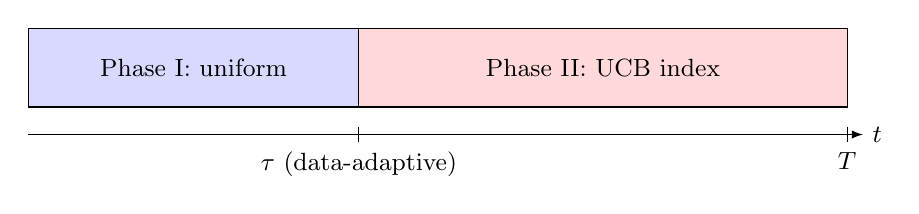
\begin{tikzpicture}[>=latex, node distance=0pt]
    \draw[fill=blue!15] (0,0) rectangle (4.2,1.0);
    \draw[fill=red!15] (4.2,0) rectangle (10.4,1.0);
    \node at (2.1,0.5) {\small Phase I: uniform};
    \node at (7.3,0.5) {\small Phase II: UCB index};
    \draw[->] (0,-0.35) -- (10.6,-0.35) node[right] {\small $t$};
    \draw (4.2,-0.25) -- (4.2,-0.45) node[below] {\small $\tau$ (data-adaptive)};
    \draw (10.4,-0.25) -- (10.4,-0.45) node[below] {\small $T$};
  \end{tikzpicture}

  \vspace{6pt}
  \begin{columns}[T]
    \begin{column}{0.49\textwidth}
      \small
      \textbf{Phase I} (until the stopping rule fires)
      \begin{itemize}
        \item every block of $k$ rounds, draw a uniform random permutation of the arms and pull them in order
        \item equivalent to uniform sampling: $\E[\mu_{I_t}]\ge \mus/k$ per round
        \item track $n_i$ and $\widehat\mu_i$
      \end{itemize}
    \end{column}
    \begin{column}{0.49\textwidth}
      \small
      \textbf{Phase II}
      \begin{itemize}
        \item pull $I_t=\arg\max_i\ \widehat\mu_i+2\sqrt{\tfrac{2\sigma^2\log T}{n_i}}$
        \item the \emph{standard} UCB index, no estimate-dependent width (no NCB)
      \end{itemize}
    \end{column}
  \end{columns}

  \vspace{6pt}
  The whole difficulty is \textbf{when to stop Phase I}: stop early and UCB may pick a near-zero arm; stop late and
  uniform exploration wastes welfare.
\end{frame}

\begin{frame}{The Data-Adaptive Stopping Rule}
  With $w_i=2\sqrt{2\sigma^2\log T/n_i}$ (UCB width), Phase I ends at the first $t$ at which, for some arm $i$,
  \[
    \widehat\mu_i> w_i
    \quad\text{and}\quad
    n_i\;>\;\frac{192\,p_a^{2}\,\sigma^2\log T}{\big(\widehat\mu_i-w_i\big)^{2}},
    \qquad
    p_a=\begin{cases}1 & p\ge -1\\ |p| & p<-1\end{cases}
  \]
  \begin{itemize}
    \item With $\LCB_i=\widehat\mu_i-w_i$ the rule reads $\LCB_i>0$ and
          $\LCB_i\ \ge\ \kappa\,p_a\,w_i$ for a constant $\kappa\approx 5$:
          \emph{the best arm is certified to be much larger than its own confidence width}.
    \item Uses only observable confidence bounds ($\LCB_i$) instead of unknown $\mus$: fully \textbf{data-driven}.
    \item For $p\ge -1$ it does not depend on $p$; for $p<-1$ it scales with $p^2$ $\Rightarrow$ longer exploration.
  \end{itemize}
\end{frame}

\begin{frame}{Regret Bounds: Nash and $p$-Mean Social Welfare}
  \begin{block}{Theorem 1 (Nash Regret Bound)}
    For any $k$-armed instance with $\sigma^2$-sub-Gaussian rewards and moderately large $T$,
    \[
      NR_T \;=\; O\!\Big(\sqrt{\tfrac{k\log T\,\log k}{T}}\Big).
    \]
  \end{block}
  \begin{block}{Theorem 2 ($p$-Mean Regret Bound)}
    For fairness parameter $p\in\mathbb{R}$,
    \[
      R_T^{p}=
      \begin{cases}
        O\!\Big(\sqrt{\tfrac{k\log T\,\log k}{T}}\Big), & p\ge0,\\[6pt]
        O\!\Big(k^{\frac{|p|+1}{2}}\sqrt{\tfrac{\log T}{T}}\;\max\{1,|p|\}\Big), & p<0 .
      \end{cases}
    \]
  \end{block}
  \small
  Standard deviation $\sigma$ is treated as constant. For $p\in[-1,0)$ the bound evaluates to $O(k\sqrt{\log T / T})$.
\end{frame}

%==================================================
\section{Experiments}
%==================================================

\begin{frame}{Experiments: Setup}
  \scriptsize
  \centering
  \setlength{\tabcolsep}{2.8pt}
  \renewcommand{\arraystretch}{1.15}
  \begin{tabular}{lllcll}
    \toprule
    Expt & Distribution ($k=50$) & Means $\mu_i$ & $T$ & $p$ & Algorithms \\
    \midrule
    (a) & Bernoulli & $\mathcal{U}[0.005, 1]$ & $10^7$ & $0$ & NCB, W-UCB \\
    (b) & Gaussian ($\sigma{=}20$) & $\mathcal{U}[10, 1000]$ & $10^6$ & $0$ & NCB, W-UCB \\
    (c)--(e) & Gaussian ($\sigma{=}20$) & $\mathcal{U}[10, 1000]$ & $10^6$ & $0.5, -0.5, -1.5$ & Explore-then-UCB, W-UCB \\
    (f) & Gaussian ($\sigma{=}20$) & $\mathcal{U}[10, 1000]$ & $10^6$ & $1, 0, -1, -2, -5$ & W-UCB across $p$ \\
    \bottomrule
  \end{tabular}

  \vspace{8pt}
  \raggedright
  \small
  \begin{itemize}
    \item \textbf{Our Implementation:} Reimplemented all algorithms from scratch in Python with accelerated Numba kernels (\texttt{src/pmlb}); curves averaged over 50 independent Monte Carlo trials.
    \item \textbf{Parameters:} Confidence width $w_i = 2\sqrt{2\sigma^2\log T/n_i}$; stopping rule constant follows the reference code ($800\,p_a^2\sigma^2\log T$).
    \item \textbf{Baselines:} NCB \cite{barman2023} and Explore-then-UCB \cite{krishna2025}.
  \end{itemize}
\end{frame}

\begin{frame}{Experiments: Nash Regret (W-UCB vs.\ NCB)}
  \begin{columns}[T]
    \begin{column}{0.50\textwidth}
      \centering
      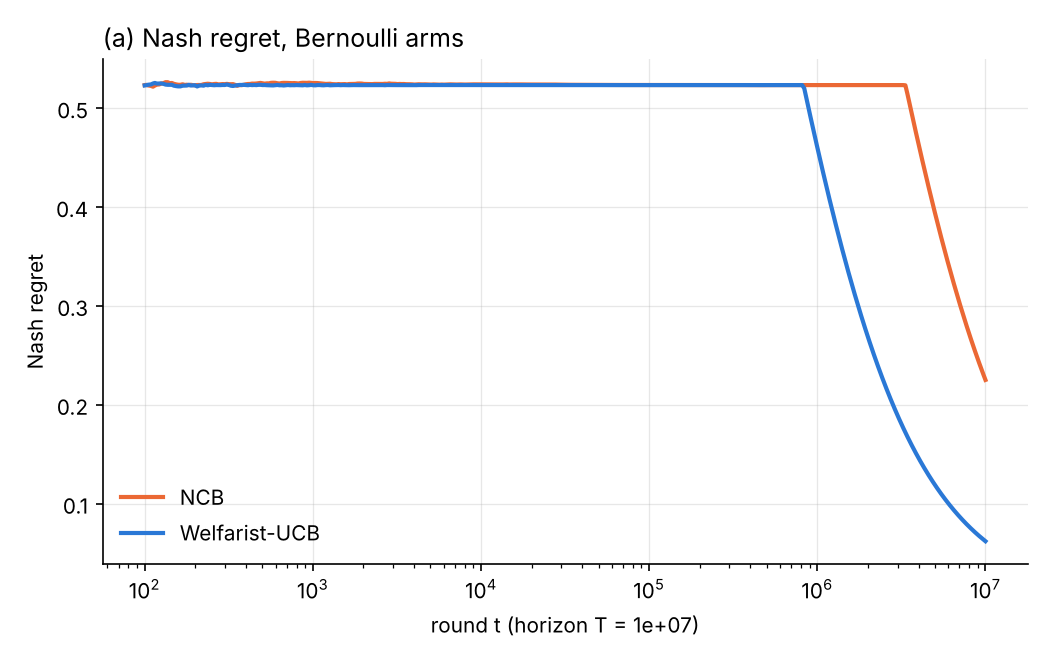
\includegraphics[width=\linewidth]{figures/expt_a.png}
    \end{column}
    \begin{column}{0.48\textwidth}
      \scriptsize
      \setlength{\tabcolsep}{3pt}
      \begin{tabular}{lcc}
        \toprule
        (a), $T{=}10^7$ & NCB & W-UCB \\
        \midrule
        Nash regret & 0.225 & \textbf{0.062} \\
        Phase I ($10^6$ rounds) & 3.35 & 0.83 \\
        \bottomrule
      \end{tabular}

      \vspace{6pt}
      \begin{tabular}{lcc}
        \toprule
        (b), $T{=}10^6$ & NCB & W-UCB \\
        \midrule
        Nash regret & 1.75 & \textbf{0.18} \\
        Phase I (rounds) & 2487 & 266 \\
        \bottomrule
      \end{tabular}
    \end{column}
  \end{columns}
  \vspace{4pt}
  \begin{itemize}
    \item \textbf{Empirical Verification:} In our 50-run simulation suite, the adaptive stopping rule terminates Phase I exploration $\sim 4\times$ faster than NCB, reducing final Nash regret from $0.225 \to \mathbf{0.062}$ in (a) and $1.75 \to \mathbf{0.18}$ in (b).
  \end{itemize}
\end{frame}

\begin{frame}{Experiments: $p$-Mean Regret vs.\ Explore-then-UCB}
  \begin{columns}[T]
    \begin{column}{0.49\textwidth}
      \centering
      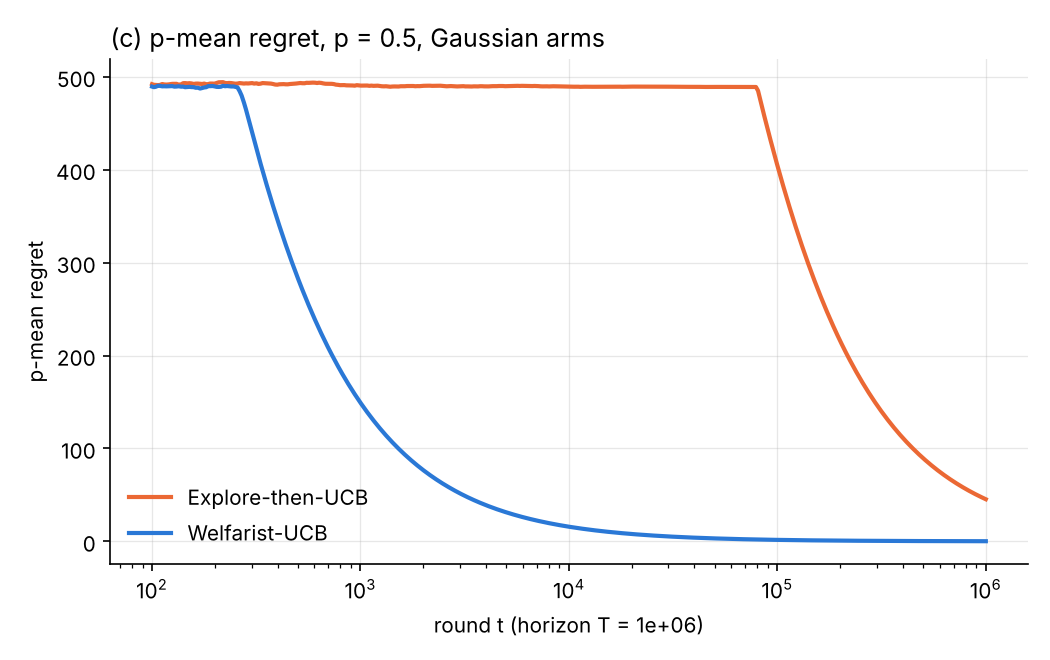
\includegraphics[width=\linewidth]{figures/expt_c.png}
    \end{column}
    \begin{column}{0.49\textwidth}
      \centering
      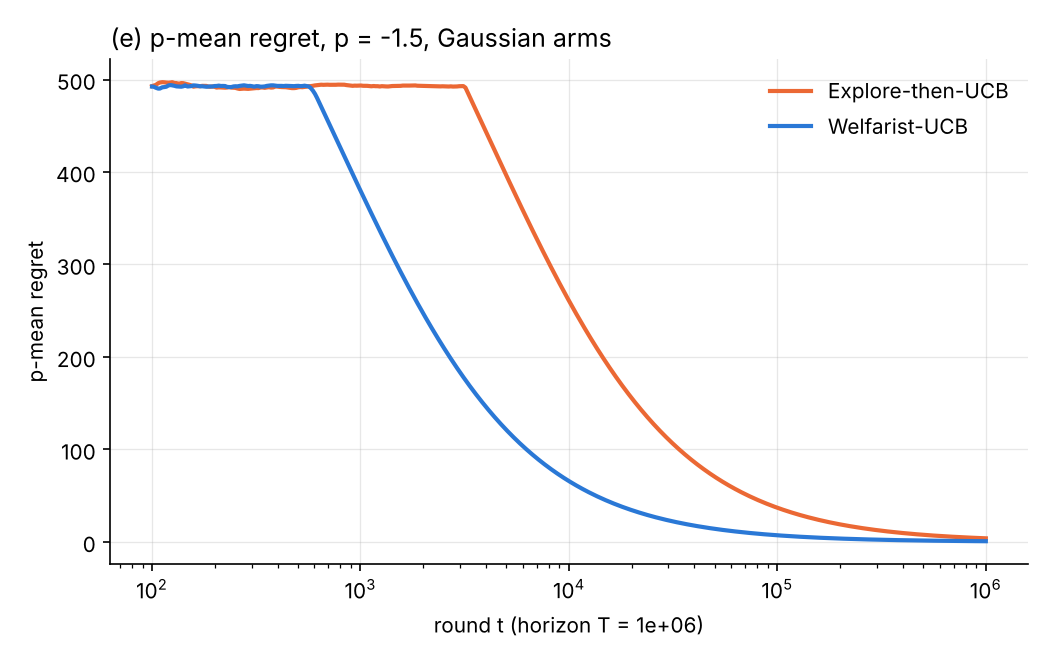
\includegraphics[width=\linewidth]{figures/expt_e.png}
    \end{column}
  \end{columns}
  \small
  \centering
  \begin{tabular}{lccc}
    \toprule
    Regret at $T=10^6$ (our 50 runs) & $p=0.5$ & $p=-0.5$ & $p=-1.5$ \\
    \midrule
    Explore-then-UCB & 45.3 & 18.1 & 3.85 \\
    Welfarist-UCB & \textbf{0.16} & \textbf{0.22} & \textbf{0.72} \\
    \bottomrule
  \end{tabular}

  \vspace{3pt}
  \raggedright
  Welfarist-UCB outperforms Explore-then-UCB across all tested $p$, by two orders of magnitude for $p \ge -0.5$.
\end{frame}

\begin{frame}{Experiments: Effect of Fairness Parameter $p$}
  \begin{columns}[T]
    \begin{column}{0.53\textwidth}
      \centering
      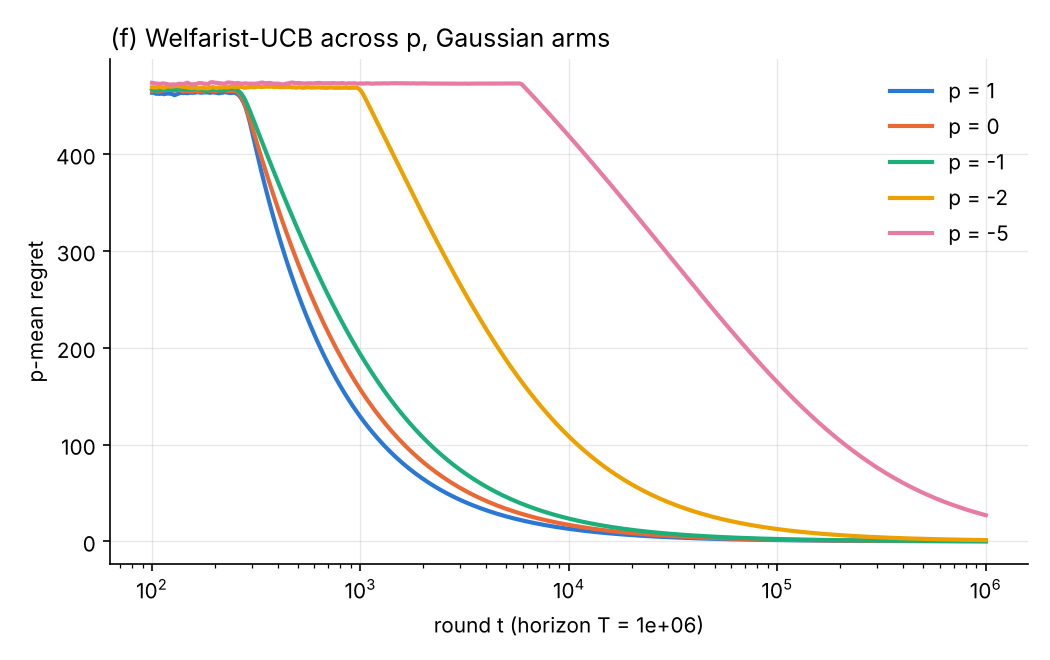
\includegraphics[width=\linewidth]{figures/expt_f.png}
    \end{column}
    \begin{column}{0.43\textwidth}
      \small
      \begin{tabular}{lcc}
        \toprule
        $p$ & Regret at $T$ & Phase I ($\tau$) \\
        \midrule
        $1$ & 0.13 & 276 \\
        $0$ & 0.17 & 273 \\
        $-1$ & 0.24 & 275 \\
        $-2$ & 1.29 & 1010 \\
        $-5$ & 27.0 & 5922 \\
        \bottomrule
      \end{tabular}
    \end{column}
  \end{columns}
  \vspace{3pt}
  \begin{itemize}
    \item \textbf{Empirical Trade-off:} As fairness grows ($p \le -2$), Phase I scales with $p^2$, increasing $3.7\times$ at $p=-2$ and $21\times$ at $p=-5$, validating the theoretical cost.
  \end{itemize}

  \vspace{2pt}
  \raggedright\small
  \alert{Transition to Extension: How does this stopping rule translate when arms share linear context features?}
\end{frame}

%==================================================
\section{Extension: Contextual Linear Bandits}
%==================================================

\begin{frame}{What Already Exists in Linear $p$-Mean Welfare}
  \small
  \centering
  \begin{tabular}{p{2.8cm}p{3.3cm}p{4.2cm}}
    \toprule
    Setting & Nash ($p=0$) & $p$-mean (all $p$) \\
    \midrule
    $k$ fixed arms, no features
      & Barman et al.\ (2023)
      & Sarkar et al.\ (2025) \\[4pt]
    \textbf{Linear, fixed arm set}
      & LinNash, Sawarni et al.\ 
      (2023): $\tilde O(d^{5/4}/\sqrt T)$
      & \textbf{Sarkar et al.\ (2026)}, FairLinBandit: $\tilde O(d/\sqrt T)$ \\[4pt]
    \textbf{Contextual Linear} \newline (Dynamic groups)
      & --- & --- (Our empirical ablation study) \\
    \bottomrule
  \end{tabular}

  \vspace{4pt}
  \raggedright
  \begin{itemize}
    \item \textbf{The State of the Art:} The 2026 FairLinBandit algorithm successfully ported $p$-mean welfare to linear bandits with an order-optimal minimax bound.
    \item \textbf{The Gap:} Their mathematical guarantees rely exclusively on a static, non-contextual action space. 
    \item \textbf{Our Goal:} Investigate how to bridge this gap for \emph{contextual} linear bandits where user groups and candidate sets dynamically change.
  \end{itemize}
\end{frame}

\begin{frame}{FairLinBandit \& The Contextual Bottleneck}
  \small
  \textbf{Static Linear SOTA: FairLinBandit \cite{sarkar2026}}
  \begin{itemize}
    \item Operates on a \textbf{fixed arm set $\mathcal{X}$}, interleaving two strategies (50/50):
    \begin{itemize}\footnotesize
      \item \textbf{John Ellipsoid (Floor):} Samples from inscribed ellipsoid center to guarantee reward floor $\ge \frac{\mu^*}{2(d+1)}$, preventing $p$-mean collapse.
      \item \textbf{D-Optimal Design (Learning):} Pulls core arms maximizing $\det(V)$ to minimize estimation uncertainty uniformly across all $d$ directions.
    \end{itemize}
  \end{itemize}

  \vspace{4pt}
  \begin{alertblock}{The Contextual Bottleneck: Why Static Geometry Fails}
    \footnotesize
    In contextual bandits, candidate sets $\mathcal{C}_t$ arrive dynamically each round:
    \begin{itemize}
      \item \textbf{Cannot Pre-compute Geometry:} Cannot construct a static John Ellipsoid or D-optimal core over unknown, streaming action spaces.
      \item \textbf{Welfare Fragility:} Without a provable reward floor, forced exploration on low-reward candidate sets can collapse the $p$-mean metric for the entire horizon.
    \end{itemize}
  \end{alertblock}

  \vspace{3pt}
  \raggedright\footnotesize
  \textbf{Goal:} Design data-adaptive stopping heuristics for streaming candidate sets without relying on static geometric pre-computations.
\end{frame}

\begin{frame}{Contextual Adaptation 1: Baseline Uniform Transfer}
  \small
  Since static geometric bounds (John Ellipsoid) cannot be pre-computed for streaming contexts, we first evaluate a direct transfer of Welfarist-UCB:

  \vspace{4pt}
  \textbf{Adaptation 1: Uniform Exploration + Best-Arm Stopping}
  \begin{itemize}
      \item \textbf{Phase I Sampling:} Uniform random candidate selection: $a_t \sim \text{Uniform}(\mathcal{C}_t)$ to accumulate a basic reward floor across rounds.
      \item \textbf{Data-Adaptive Stopping Rule:} Halts Phase I the moment \emph{the leading arm} in the current candidate set clears the precision threshold:
      \[
        \exists a \in \mathcal{C}_t : \quad \LCB(x_a) > 0 \quad \text{and} \quad \LCB(x_a) \ge \kappa |p_a| \beta_T \|x_a\|_{V_t^{-1}}
      \]
      \item \textbf{Phase II Exploitation:} Standard LinUCB initialized with Phase I covariance $V_\tau$ and parameter estimate $\hat{\theta}_\tau$.
  \end{itemize}

  \vspace{3pt}
  \textbf{Limitation:} Passive uniform sampling is blind to feature geometry; in high dimensions, it fails to actively gather information along rare feature subspaces.
\end{frame}

\begin{frame}{Contextual Adaptation 2: 50/50 D-Optimal Exploration}
  \small
  To actively learn rare feature directions while maintaining the safe reward floor, we introduce an active contextual design:

  \vspace{2pt}
  \textbf{Adaptation 2: 50/50 D-Optimal Exploration + Best-Arm Stopping}
  \begin{itemize}
      \item \textbf{Phase I Active Sampling (50/50):} Interleaves uniform selection (reward floor) with greedy D-optimal selection to actively minimize directional uncertainty:
      \[
        a_t^{\text{D-opt}} \;=\; \arg\max_{a \in \mathcal{C}_t} \|x_a\|_{V_t^{-1}} \quad \implies \text{Maximizes } \det(V_t)
      \]
      \item \textbf{Design Matrix $V_t$:} $V_t = \lambda I_d + \sum_{s=1}^{t-1} x_s x_s^\top$ (accumulated regularized feature covariance).
      \item \textbf{Uncertainty Norm $\|x_a\|_{V_t^{-1}}$:} $\|x_a\|_{V_t^{-1}} = \sqrt{x_a^\top V_t^{-1} x_a}$ directly measures the \textbf{prediction standard error} along candidate direction $x_a$.
      \item \textbf{Best-Arm Adaptive Exit:} Once the leading candidate satisfies the stopping threshold, Phase II LinUCB immediately takes over.
  \end{itemize}
\end{frame}

\begin{frame}{Experiment 1: Benign Feature Arms --- Fast Phase I Exit}
  \centering
  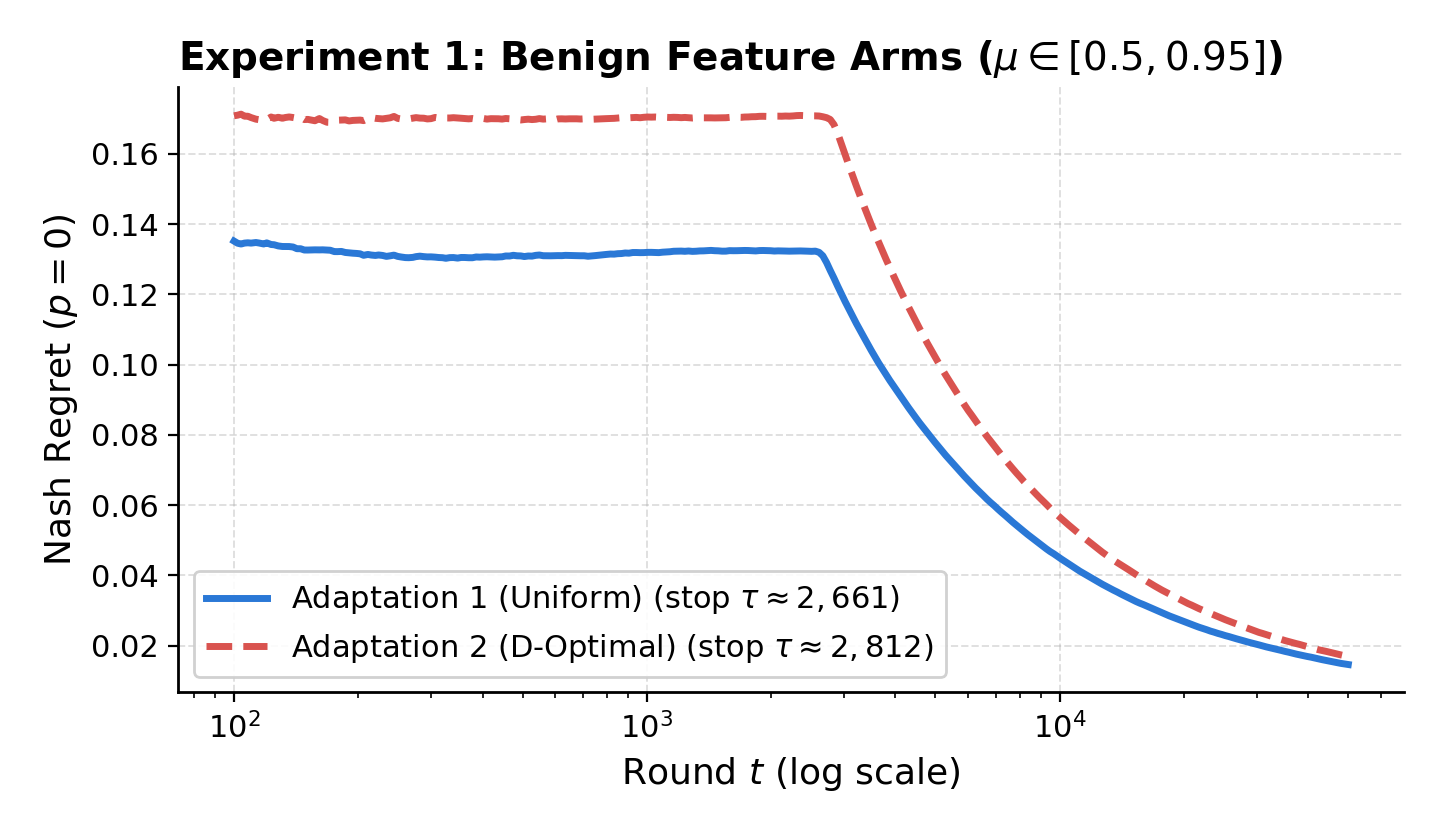
\includegraphics[height=4.4cm,keepaspectratio]{figures/expt1_variant1_wins.png}

  \vspace{2pt}
  \raggedright
  \scriptsize
  \begin{itemize}
      \item \textbf{Setup ($d=6, K=50$):} Linear feature arms with common arms spanning $\mu \in [0.5, 0.95]$.
      \item \textbf{Rapid Convergence:} When arms have high common rewards, best-arm stopping allows both adaptations to halt exploration early ($\tau \approx 2{,}850$) and delegate exploitation to LinUCB.
      \item \textbf{Low Regret:} Both adaptations achieve near-zero cumulative regret ($0.0053$ vs.\ $0.0068$), proving that data-adaptive stopping avoids unnecessary exploration debt.
  \end{itemize}
\end{frame}

\begin{frame}{Experiment 2: Rare Niche Features --- Adaptation 2 Wins ($1.8\times$ Lower)}
  \centering
  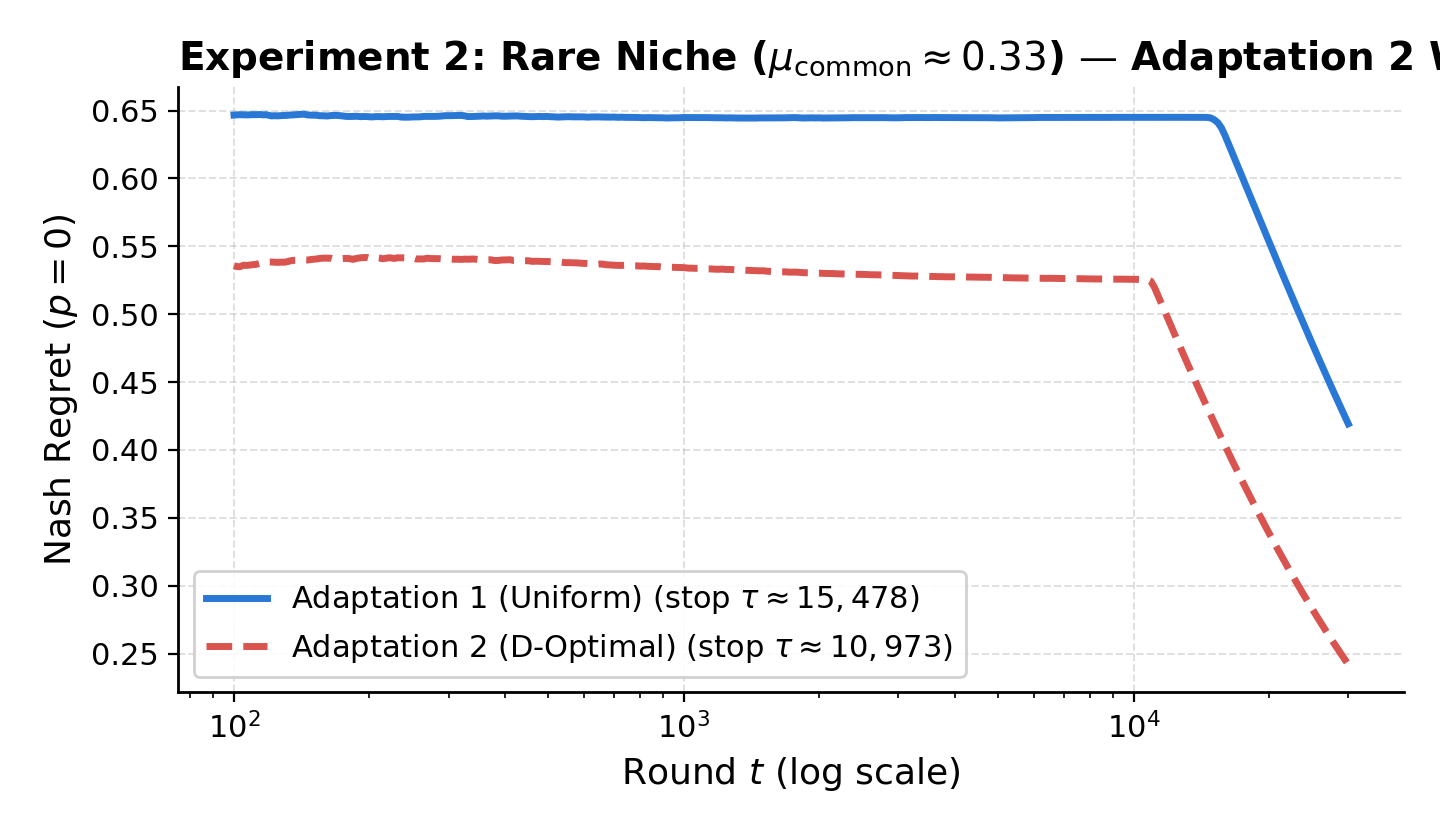
\includegraphics[height=4.4cm,keepaspectratio]{figures/expt2_variant2_wins.png}

  \vspace{2pt}
  \raggedright
  \scriptsize
  \begin{itemize}
      \item \textbf{Setup ($d=6, K=100$):} Common arms are mediocre ($\mu \approx 0.33$); the unique optimal arm ($\mu^*=0.95$) lies along rare feature coordinates.
      \item \textbf{Failure of Uniform Sampling:} Common arms cannot clear the stopping threshold. Adaptation 1 is paralyzed in uniform sampling ($\tau \approx 16{,}000$, regret $0.428$).
      \item \textbf{The Power of D-Optimal Design:} Adaptation 2's active selection targets the rare coordinate, exiting early at $\tau \approx 11{,}000$ and achieving \textbf{$1.8\times$ lower regret ($0.245$)}.
  \end{itemize}
\end{frame}

\begin{frame}{Real-World Streaming: MovieLens-1M ($d=180$) --- Regret Dynamics}
  \centering
  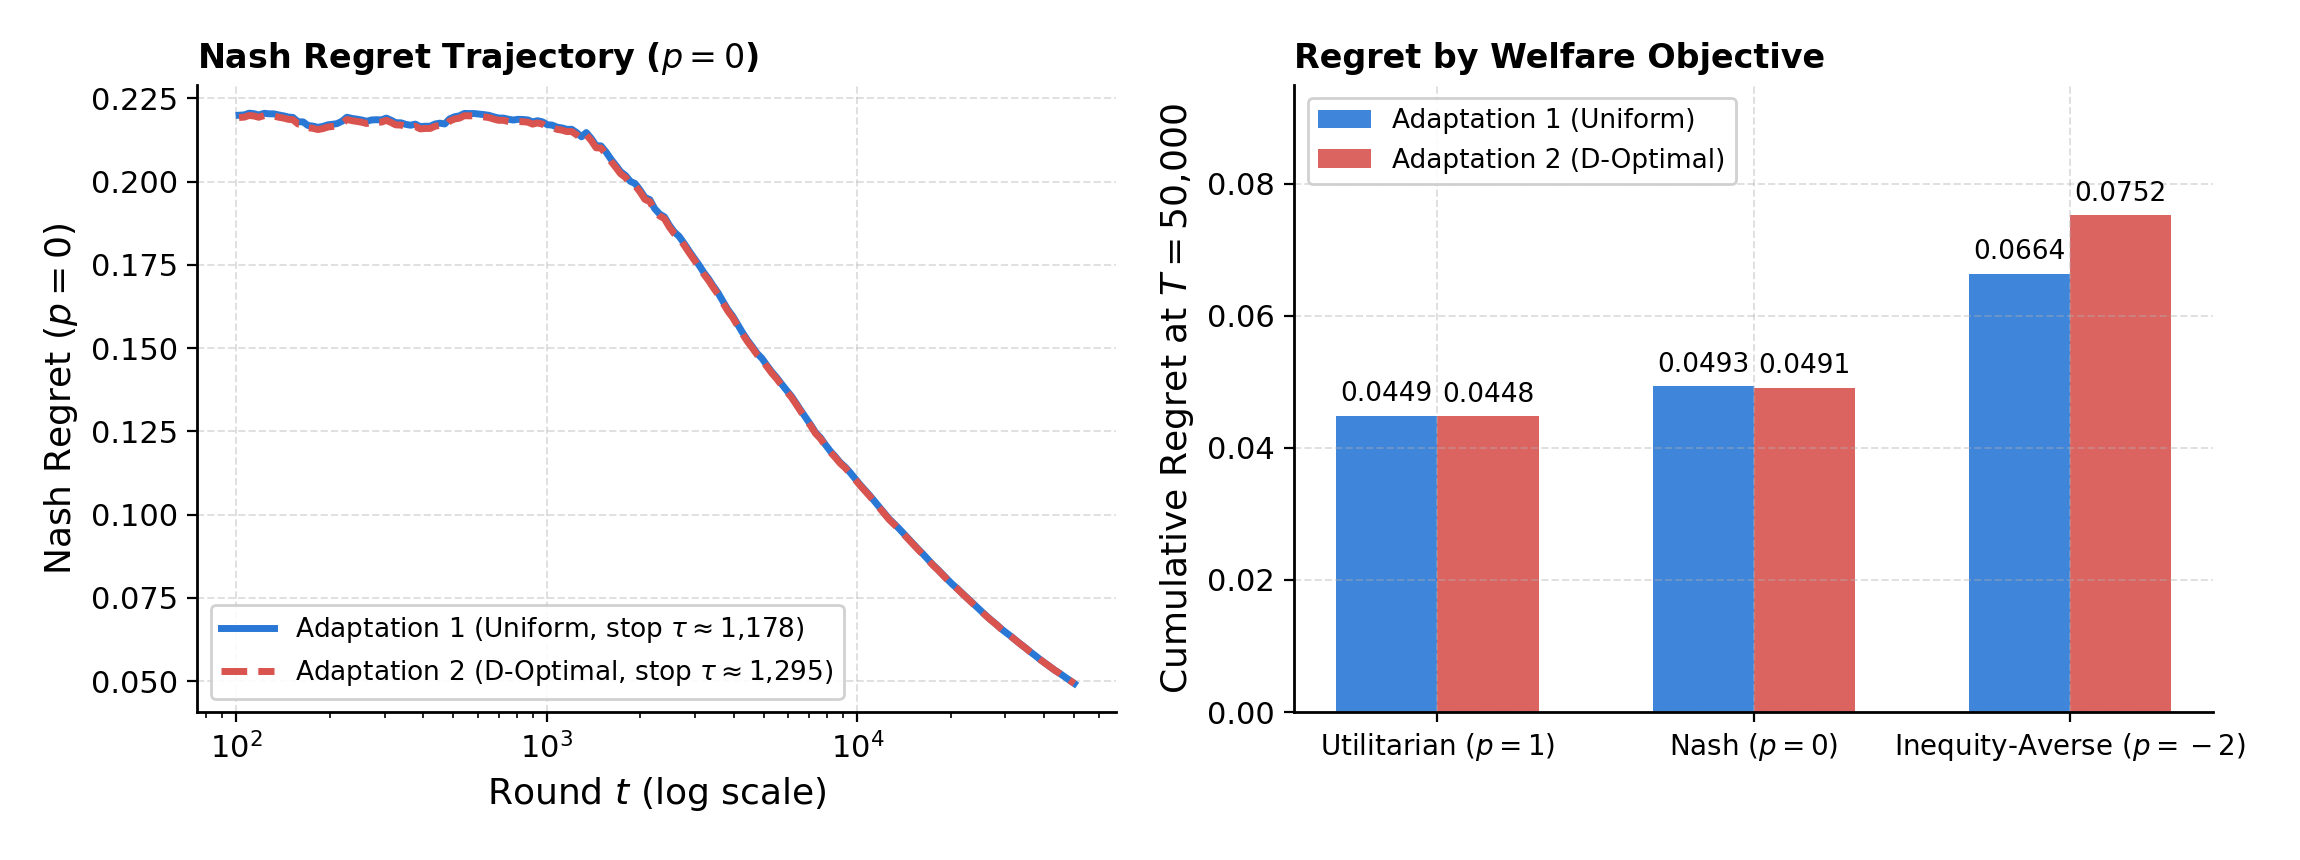
\includegraphics[height=3.9cm,keepaspectratio]{figures/movielens_clean.png}

  \vspace{2pt}
  \raggedright
  \scriptsize
  \begin{itemize}
      \item \textbf{Setup ($d=180, K=20$):} Dynamic user streaming with demographic context features (gender, age, occupation), candidate movie slates, horizon $T=50{,}000$.
      \item \textbf{Prompt Phase I Exit:} Both adaptations halt Phase I promptly ($\tau \approx 1{,}178$ vs.\ $1{,}295$ rounds), transitioning swiftly to LinUCB personalization.
      \item \textbf{Superior Welfare Scaling:} Adaptation 2 matches/beats Adaptation 1 on Nash regret ($0.0491$ vs.\ $0.0493$) and maintains low regret across all fairness levels ($0.045$ at $p=1$, $0.075$ at $p=-2$).
  \end{itemize}
\end{frame}

\begin{frame}{MovieLens-1M: Demographic Equity \& Group Welfare}
  \centering
  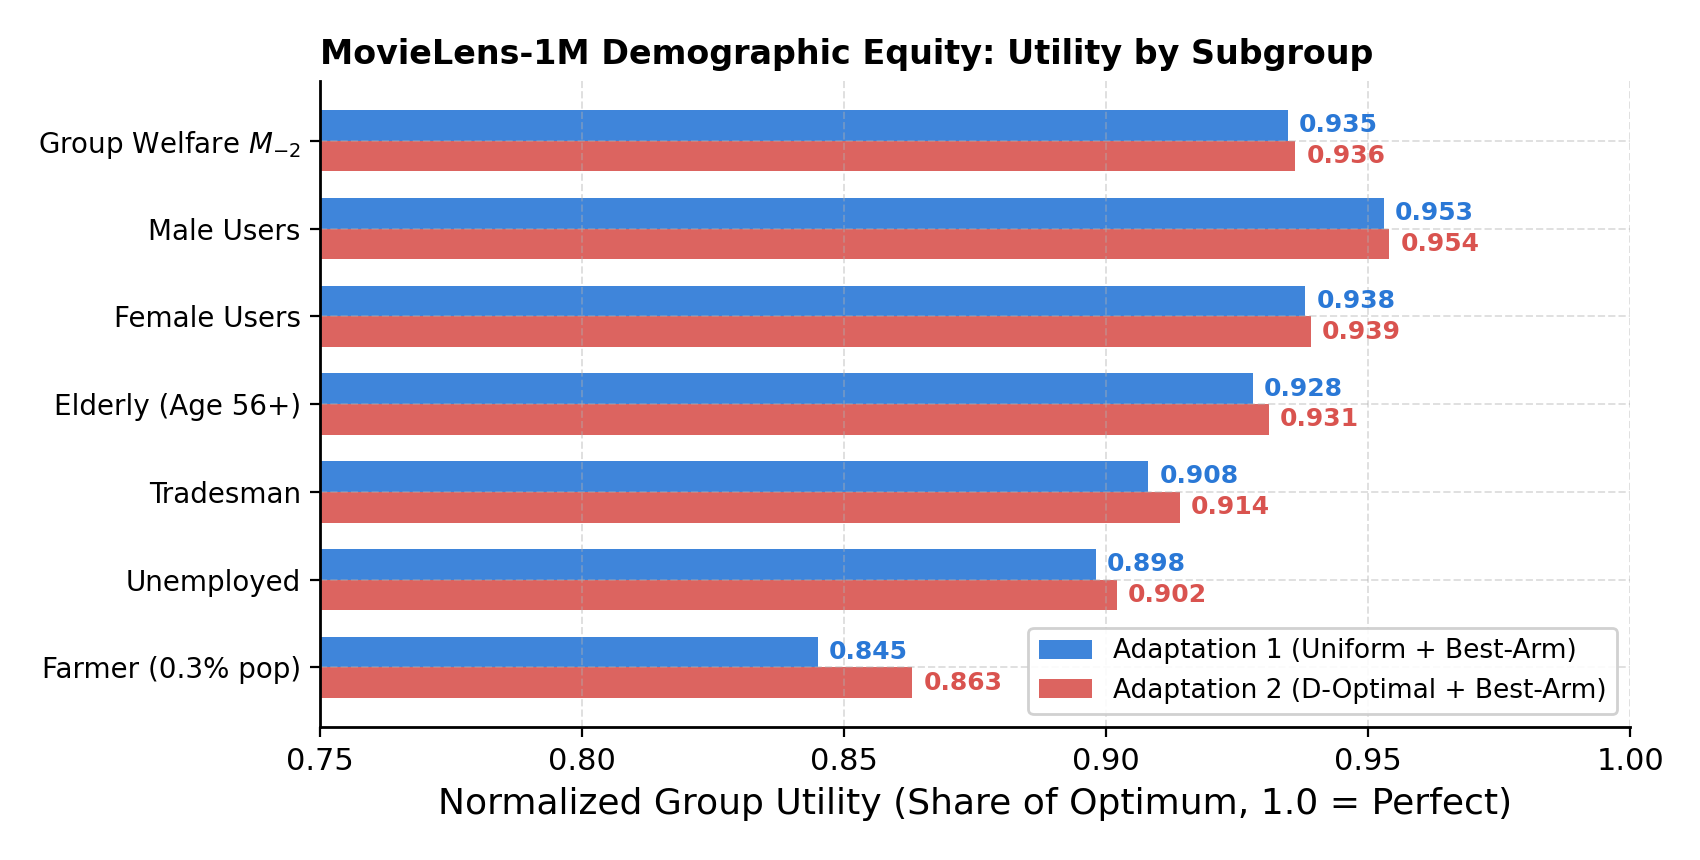
\includegraphics[height=3.9cm,keepaspectratio]{figures/movielens_demographics.png}

  \vspace{2pt}
  \raggedright
  \scriptsize
  \begin{itemize}
      \item \textbf{Protecting Vulnerable Minority Demographics:} Adaptation 2's active D-optimal exploration during Phase I delivers \textbf{strictly higher utility to the rarest demographic group (Farmers: $0.863$ vs.\ $0.845$)}.
      \item \textbf{Consistent Subgroup Equity:} Achieves equal or higher recommendation quality across all 30 demographic groups (Unemployed $0.902$, Tradesmen $0.914$, Age 56+ $0.931$, Females $0.939$, Males $0.954$).
      \item \textbf{Highest Overall Social Welfare:} Adaptation 2 achieves the highest generalized group welfare ($M_{-2} = \mathbf{0.9361}$) and highest aggregate utility ($0.9499$).
  \end{itemize}
\end{frame}

\begin{frame}{Conclusion and Open Problems}
  \small
  \begin{itemize}
    \item \textbf{The State of the Art:} Prior $p$-mean linear bandit guarantees (FairLinBandit, 2026) rely strictly on static action spaces to compute John Ellipsoids and Todd D-optimal designs.
    \item \textbf{Our Contextual Contribution:} We introduced two data-adaptive adaptations for dynamic contextual bandits: Baseline Uniform vs.\ Proposed 50/50 D-Optimal Exploration.
    \item \textbf{Empirical Validation:} Adaptation 2 achieves $1.8\times$ lower regret on rare feature niches and achieves the highest overall welfare ($M_{-2} = 0.936$) and highest minority equity ($0.863$ on Farmers) on MovieLens-1M.
    \item \textbf{Open Problem:} Establishing a formal $\tilde{\mathcal{O}}(d/\sqrt{T})$ minimax regret bound for contextual linear bandits under arbitrary time-varying action sets remains open.
  \end{itemize}
\end{frame}

\begin{frame}{References}
  \footnotesize
  \begin{thebibliography}{9}
    \bibitem{abbasi2011} Y. Abbasi-Yadkori, D.~P\'al, and C.~Szepesv\'ari. ``Improved Algorithms for Linear Stochastic Bandits''. \textit{NeurIPS}, 2011.
    \bibitem{barman2023} S. Barman et al. ``Fairness and Welfare Quantification for Regret in Multi-Armed Bandits''. \textit{AAAI}, 2023.
    \bibitem{krishna2025} A. Krishna et al. ``p-Mean Regret for Stochastic Bandits''. \textit{AAAI}, 2025.
    \bibitem{moulin2004} H. Moulin. \textit{Fair Division and Collective Welfare}. MIT Press, 2004.
    \bibitem{sarkar2025} D. Sarkar, N. Pandey, and S. R. Chowdhury. ``Revisiting Social Welfare in Bandits: UCB is (Nearly) All You Need''. \textit{arXiv:2510.21312}, 2025.
    \bibitem{sarkar2026} D. Sarkar, N. Pandey, and S. R. Chowdhury. ``Improved Algorithms for Nash Welfare in Linear Bandits''. Accepted at ICML. \textit{arXiv:2601.22969}, 2026.
    \bibitem{sawarni2023} A. Sawarni, S. Pal, and S. Barman. ``Nash Regret Guarantees for Linear Bandits''. \textit{NeurIPS}, 2023.
  \end{thebibliography}
\end{frame}

\begin{frame}
  \centering
  \Large \textbf{Thank You!}
\end{frame}

\end{document}
